\chapter{Wissenschaftliche Disziplin}
\section{Chemie}
Die Funktionsweise eines Nudges wird aus der chemischen Sicht mit der Benutzung eines Katalysators bei der Durchführung eines chemischen Prozesses gleichgesetzt. Um einen chemischen Prozess zum Laufen zu bringen wird eine bestimmte Menge an Energie vorausgesetzt, die Aktivierungsenergie genannt wird. Die Aktivierungsenergie wird ebenfalls energetische Hürde genannt, da diese überschritten werden muss, damit die chemische Reaktion stattfinden kann. Es gibt zwei Arten von Katalysatoren, den positiven Katalysator und den negativen Katalysator. Hierbei setzt der positive Katalysator die Aktivierungsenergie herab und beschleunigt dadurch die Reaktion. Auf der anderen Seite erhöht ein negativer Katalysator die Aktivierungsenergie und verlangsamt dadurch die Reaktion.

Diese Aktivierungsenergie wird zum Beispiel als Wärmeenergie zugeführt, was an folgendem Versuchsaufbau zu erkennen ist.
Wird Wasserstoff mit Sauerstoff in einem Verhältnis von 2:1 in einem Ballon, passiert nichts weiter, als dass dieser anfängt zu schweben. Das liegt daran, dass die Aktivierungsenergie, die benötigt wird, um die Stoffe miteinander reagieren zu lassen, nicht bereitgestellt wird. Die Raumtemperatur reicht hierbei nicht aus. Wird allerdings Wasserstoffgas auf einen Platinkatalysator zugeführt, agiert dieses als positiver Katalysator und verringert die energetische Hürde, sodass der chemische Prozess bei Raumtemperatur stattfinden, und das Wasserstoff sich mit dem in der Luft befindenden Sauerstoff entzündet. 

Auf folgendem Bild ist die Veränderung der energetischen Hürde durch die Zugabe eines Katalysators dargestellt:

\begin{figure}[ht]
    \centering
    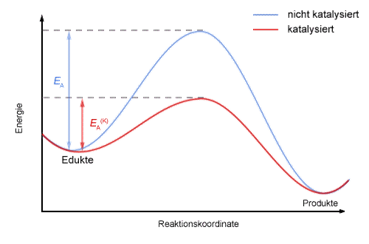
\includegraphics[width=0.9\textwidth]{Bilder/Chemie.png}
    \caption{Abgerufen von \url{http://www.chemgapedia.de/vsengine/vlu/vsc/de/ch/13/vlu/kinetik/katalyse/katalyse.vlu.html}}
    \label{fig:chemie}
\end{figure}

Es gibt im menschlichen Körper ebenfalls viele Chemische Reaktionen, welche durch Katalysatoren unterstützt werden. Diese biologischen Katalysatoren sind oftmals Enzyme welche zum Beispiel im Speichel den Prozess des Verdauens unterstützen.

Übertragen ins Psychologische kann eine chemische Reaktion als physische Handlung eines Menschen betrachtet werden. Hierbei stellt die energetische Hürde die Tatkraft eines Menschen die betroffene Handlung durchzuführen. Nudges sind als Katalysatoren zu verstehen, die in Form von positiven Nudges die Durchführung der Handlung fördern oder als negativer Nudge die Durchführung hemmen wollen. Bei einem positiven Nudge wird zum Beispiel durch das Bereitstellen von günstigeren Gegebenheiten für das Wählen der Handlung gesorgt. Dadurch sinkt die energetische Hürde und die Wahrscheinlichkeit, dass diese Handlung durchgeführt wird, ist größer.

\section{Psychologie}
\subsection{Libertärer Paternalismus}
Der Libertärer Paternalismus ist eine zugrundeliegende Philosophie des Nudgings und dient gleichzeitig als dessen Leitphilosophie. Somit sollten sich auch Unternehmen, die Nudging benutzen und das Denken der Menschen zu ihrem Vorteil beeinflussen, mir diesem Ansatz vertraut machen.
Der Begriff „Libertär“ steht für die Freiheit der Menschen und ihrer Entscheidungen. Er wird als Zusatz verwendet, um den Begriff Paternalismus so zu erweitern, dass dieser als freiheitserhaltend verstanden wird. Dies ist besonders bei einem weitreichenden und einflussreichen Konzept wie Nudging wichtig. Die Nudge-Theorie entstand mit dem Hintergrund, den Beeinflussten eine Hilfestellung bei Entscheidungen zu geben. Jedoch wird der Ansatz in der heutigen Zeit vermehrt zur Gewinnsteigerung von Konzernen, bzw. zur Verfolgung eigennütziger Ziele verwendet. Dabei betonen Thaler und Sunstein auch, dass sich Menschen einfacher und effizienter beeinflussen lassen, wenn sie Sympathie für den Einsetzenden der Nudges empfinden. Es ist demnach durchaus im Interesse der Einflussnehmenden, den Nudge unauffällig einzusetzen und im Gesamteindruck ein positives Image zu hinterlassen. Dieser Zusammenhang wird nicht direkt in dem Buch der beiden Professoren erwähnt, jedoch fügten sie im Nachhinein an, dass es einen elementaren Teil der Nudge-Theorie ausmacht \parencite{Businessballs.2013}. In dem folgenden Kapitel wird der Einsatz der Nudge-Theorie und deren Wirkung bei Menschen eingegangen. 

\subsection{The Choice Architect}
Der Begriff “Choice Architect” bezeichnet eine Führungskraft, eine Person oder eine Gruppe, welche in der Verantwortung steht, die Nudge Theorie einzusetzen.

Wie aus der Terminologie zu erkennen ist, stellt der Choice Architect die Entscheidungsmöglichkeiten des Nudges zur Auswahl. Darunter befindet sich, meistens hervorgehoben, auch die gewünschte Auswahloption. Das Ziel des Choice Architect ist es, die Mehrheit der Beeinflussten zur Wahl dieser Option zu verleiten, bzw. zu nudgen. Ein wichtiges Element des Nudging ist es, dass die finale Entscheidung von dem beeinflussten Menschen, und nicht vom Choice Architect getroffen wird. Diese Entscheidung wird in einer Mehrheit der Fälle unterbewusst getroffen. Obwohl Thaler und Sunstein nicht explizit darauf hingewiesen, dass der Choice Architect ethisch und angemessen seine Rechenschaftspflicht ausgeübt werden soll, haben beide deutlich gemacht, dass der ethische Einsatz für das Konzept des Nudgings essenziell ist.

Die Anpassung eines Nudges auf einzelne Menschen kann nicht präzise erfolgen, wenn die Zielgruppe eine größere Bevölkerungsmassen ist. Meistens entscheiden sich Choice Architects in solchen Szenarien für die Verwendung bekannter und einflussreicher Personen. So wird beispielsweise das Verhalten Dalai-Lamas eingesetzt, wenn man Meschen bei Entscheidungen über ihr Wohlbefinden beeinflussen möchte. Dies liegt vor allem daran, dass der Großteil der Menschen die Figur des Dalai-Lama mit einem gesunden Lebensstil verknüpfen. Wenn jedoch Menschen dazu bewegt werden sollen, mehr Aktivität in ihr Leben einzubauen, wird Michael B Jordan, ein bekannter amerikanischer Schauspieler, als Werbepersönlichkeit gewählt. Dieser wird von Vielen als sportliches Vorbild angesehen.

\subsection{Wie denkt der Mensch? Nutzung von Heuristiken zur Analyse}
In den ersten Seiten ihres Buches gehen Thaler und Sunstein auf die Fragen ein, warum sich Menschen wie im Vorherigen Kapitel beschreiben, beeinflussen lassen. Zudem wird dort beantwortet, warum Beeinflusste mehr auf Nudges von vertrauten Personen reagieren. Im Folgenden wird die Thematik der Entscheidungsfindung aufgearbeitet, und Rückschlüsse auf die Funktionsweise von Nudging gezogen.

Heuristiken sind das Einsatzmittel, mit dem Nudging funktioniert. In ihrer Nudge Theory haben Thaler und Sunstein fünfzehn verschiedene Arten der Heuristiken vorgestellt. Im Folgenden werden fünf davon näher betrachtet \parencite{Businessballs.2013}.

Wie auch bei der Project Theory spielt auch hier die „Loss Aversion“ eine große Rolle. Hier geht es darum, dass Menschen ein Verlust mehr trifft als einen Gewinn. Dies passiert auch, wenn der Gewinn deutlich höher ist als der Verlust. Dies ist einer der Gründe, warum Menschen dazu tendieren, auch bei hoher Gewinnchance und nur geringer Chance auf Verlust, die sicherere Variante zu nehmen. Es erscheint Vielen logischer nur einen kleinen  bis gar keinen Gewinn einzuholen, dafür aber auf das Risiko des Verlustes zu verzichten \parencite[]{Thaler.2021}.

Eine andere Heuristik ist die des „Status quo Voreingenommenheit und Trägheit“. Hier wird auf die Trägheit der Menschen eingegangen, welche Meschen dazu verleitet,  eine Situation zu akzeptieren, anstatt aktive Veränderungen vorzunehmen. Auch die Faulheit das Kleingedruckte zu lesen oder neue Arten des Lernens auszuprobieren, gehört zu dieser Heuristik. Viele Menschen kennen dieses Verhalten durch die Organspende Regel in Deutschland. Diese ist standartmäßig für jeden Deutschen so festgelegt, dass Bürger keine Organspender sind. Dies nennt sich das Opt-in-System \parencite{ApothekeAdhoc.2017}. Obwohl die Zahl der Menschen mit Bedarf auf ein Spendeorgan 12.000 beträgt, und drei Menschen pro Tag aufgrund von einem Mangel versterben \parencite{ApothekeAdhoc.2011}, ist die Quote an Menschen mit ausgefülltem Organspendeausweis unverändert niedrig. Dies liegt unteranderem daran, dass viele Deutsche nicht automatisch einen Organspendeausweis besitzen, mit dem sie bei deren Ableben als Organspender identifiziert werden können. Die meisten Personen gehen nicht den Aufwand ein, sich bewusst einen Spendeausweis zu holen, auch wenn prinzipiell eine Zustimmung zur Organspende vorhanden wäre. 

Die dritte Heuristik, welche im Rahmen dieser Arbeit beleuchtet wird, ist die Selbstkontroll-Strategie. Diese bezieht sich auf einzelne Personen, welche sich den Heuristiken bewusst sind und deshalb versuchen genau gegensätzlich zur gewünschten Reaktion zu handeln. Dies führt im Umkehrschluss zu einer eigenen Heuristik.
Im Gegensatz dazu steht der Herden-Effekt. Bei diesem hat der Mensch das Bedürfnis ein Teil eines Größeren zu sein und damit die Stärke der Masse mitzunutzen. Grundlage für das Verhalten ist die Suche nach Bestätigung von anderen. Beispiele hierfür lassen sich vor allem im Internet beobachten. Hier fühlen sich Menschen aus verschiedenen Grünen wohler als im echten Leben. Vor allem, da sie hier ein Teil einer großen Bewegung sein können, was im regionalen Umfeld den meisten nicht möglich ist.

Feedback ist die letzte, und gleichzeitig eine der wichtigsten Heuristiken. Viele Menschen kommen gerade auf der Arbeit mit der Heuristik des Feedbacks in Berührung. Beispielsweise, wenn ein Feedbackbogen ausgefüllt oder ein Mitarbeitergespräch geführt wird. Sobald die Erhebung eines Feedbacks angekündigt wird, tendieren Menschen dazu sich besser zu verhalten. Diese unbewusste Verhaltensänderung hat das Ziel, einen besseren Eindruck zu vermitteln und ein besseres Feedback zu bekommen. 
Andere Heuristiken, auf welche im Folgenden nicht näher eingegangen wird, sind Verankerung und Anpassung, Verfügbarkeit, Repräsentativität, Optimismus, Framing, Versuchung, Spotlight-Effekt, Priming, Choice Architect.
